%PLANO TCC 2016/02 change by Tiago heinrich
%------------------------------------------------
%------------------------------------------------
%j
\documentclass[11pt]{article}
\usepackage[brazil]{babel}
\usepackage[utf8]{inputenc}
%5\usepackage[latin1]{inputenc}
%\usepackage[utf8]{inputenc}
\usepackage{setspace}
\usepackage{epsfig}
\usepackage[pdftex]{hyperref}
\usepackage{multirow,multicol}
\usepackage{fancyhdr,url} 

\usepackage{authblk}%affil , para colocar a universidade

%%%%%%%%%%%%%%count enumarete start in zero
\usepackage{enumitem}
\setlist[enumerate,1]{start=1} % only outer nesting level

%%%%%%%%cite inside enumerate
\makeatletter
\newcommand{\mylabel}[2]{#2\def\@currentlabel{#2}\label{#1}}
\makeatother

%%apalike reference
%\usepackage{natbib}
\usepackage{apalike}


%\oddsidemargin -0.7cm 
%\evensidemargin -0.7cm
\topmargin -2.0cm 
%\headheight 0  cm 
\headsep 1.5cm   
%\hoffset -1.0cm
%\footskip 40pt
%\textheight = 235mm \textwidth 185mm
\oddsidemargin 0.4cm 
\evensidemargin 0.4cm
\textheight = 235mm \textwidth 165mm


\pagestyle{plain}
\usepackage{multicol}
\addtolength\columnsep{2pt}


\begin{document}
\pagestyle{fancy}
%\lhead{
\includegraphics[width=0.3\columnwidth]{figuras/logo_dcc.png}}
\lhead{
  
\includegraphics[scale=0.75]{figuras/logo_dcc.pdf}
}
\chead{
  \scriptsize{
    UNIVERSIDADE DO ESTADO DE SANTA CATARINA -- UDESC\\
    CENTRO DE CIÊNCIAS TECNOLÓGICAS -- CCT\\
    DEPARTAMENTO DE CIÊNCIA DA COMPUTAÇÃO -- DCC
  }
}
%\rhead{
\includegraphics[width=0.3\columnwidth]{figuras/logo_udescjlle.png}}
\rhead{
  
\includegraphics[scale=0.75]{figuras/logo_udescjlle.pdf}
}

\title{
Plano de Trabalho de Conclusão de Curso\\
Otimização de Motor de Jogos Através de Modelos Orientados a Dados
}

\onehalfspacing %espaçamento de 1,5

\author{UDESC -- Centro de Ciências Tecnológicas\\
Departamento de Ciência da Computação\\
Bacharelado em Ciência da Computação -- Integral\\
Turma 2013/2 -- Joinville/SC
}

\affil{
\textbf{Vinícius Bruch Zuchi} -- \texttt{vinicius.b.zuchi@gmail.com}\\
\textbf{André Tavares da Silva} -- \texttt{andre.silva@udesc.br} {\it (orientador)}%\\
%$<$Nome do Coorientador -- \texttt{email@coorientador} {\it (coorientador)}$>$ (se for o caso)
}


\date{3 de Abril de 2017}

\maketitle


%\singlespacing  %espaçamento simples
\onehalfspacing  %espaçamento de 1,5
%\doublespacing  %espaçamento duplo

%------------------------------------------------
%------------------------------------------------
%------------------------------------------------
%------------------------------------------------
%------------------------------------------------
\begin{abstract}
   Devido à grande diferença de desempenho entre os microprocessadores e a velocidade de acesso à memória principal, 
   muitas aplicações de computador modernas têm sofrido com um problema conhecido como gargalo do processador-memória, 
   no qual o processador fica ocioso aguardando dados serem buscados na memória. Aplicações gráficas, 
   principalmente jogos eletrônicos, são notórias por sofrerem deste problema pela grande quantidade de elementos 
   diferentes que as constituem. Este trabalho propõe a implementação de um motor de jogo (uma \textit{engine}), utilizando um 
   conceito relativamente novo de programação, a modelagem orientada a dados, com a finalidade de amenizar este problema de 
   acesso constante à memória.
    \textbf{Palavras-chave:} \textit{\textit{Modelagem Orientada a Dados (MOD). Motor de Jogos. Coerência de Cache} }
\end{abstract}

%------------------------------------------------
\section{Introdução e Justificativa}
\label{sec:int}

Nas últimas décadas, os microprocessadores tiveram um enorme avanço em termos de performance. A função deste componente
essencial para os computadores modernos, que por vezes também é chamado de CPU (\textit{Central Process Unit}), é 
a de processar as instruções e os dados de todos os programas presentes no computador~\cite{Clements:2006:PCH:1214951}.

Além de executar essas instruções, o microprocessador está constantemente lendo e escrevendo dados na 
memória principal, a memória RAM (\textit{Random Access Memory})~\cite{Clements:2006:PCH:1214951}. Sem essa possibilidade 
de leitura e escrita, os programas de computador por si só não teriam muitas utilidades, e sistemas complexos não poderiam 
existir.

Porém, há um problema na comunicação entre o processador e a memória: ela não é instantânea. Um sistema no qual a memória 
pode fornecer qualquer dado para o processador instantaneamente não é factível. Por este motivo, sistemas de memória são 
projetados utilizando uma hierarquia, na qual a memória é dividida em diferentes camadas, cada uma com uma capacidade de 
armazenamento maior, porém com um tempo de acesso maior do processador~\cite{Mahapatra:1999:PBP:357783.331677}, a 
figura~\ref{memhier} demonstra essa hierarquia em ordem decrescente de velocidade. 

\begin{figure}[h!]
    \centering
    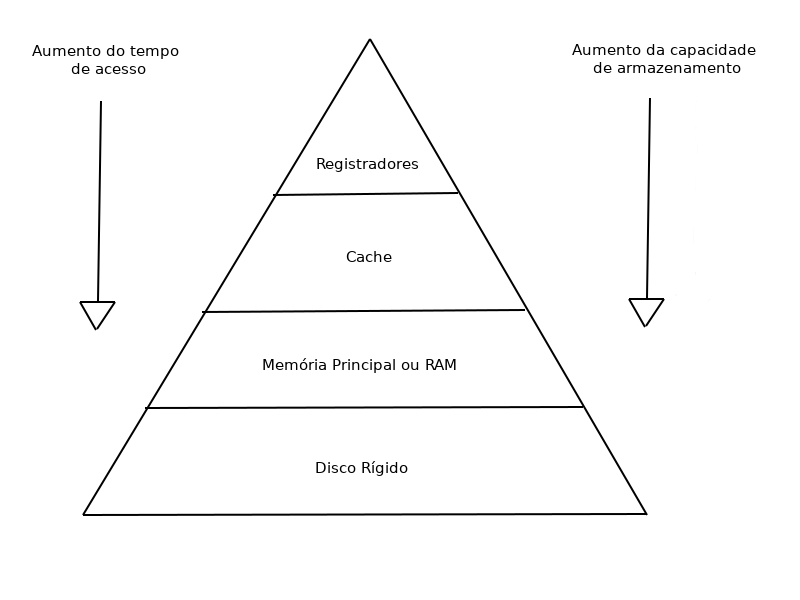
\includegraphics[width =.6\textwidth]{figuras/memoryhierarchy}
    \caption{A hierarquia do sistema de memória.}
    Fonte: Autoria própria.
    \label{memhier}
\end{figure}

As camadas do sistema de memória estão descritas a seguir: 

\begin{itemize}
    \item Registradores: são as porções da memória com o acesso mais rápido, porém em menor quantidade e com 
        pouca capacidade de armazenamento. São localizadas dentro do processador, e os compiladores são os responsáveis 
        por administrar os dados que ficam armazenados nos registradores~\cite{Clements:2006:PCH:1214951}.
    \item Cache: localizado próximo ao processador, fornece velocidade de acesso rápida e armazena código e dados utilizados 
        recentemente. Quando o processador tenta acessar algum dado presente no cache, ocorre um acerto do cache 
        (\textit{cache hit}), quando o dado não se encontra no cache, ocorre um erro do cache (\textit{cache miss}), e o dado 
        precisa ser buscado na memória principal~\cite{Mahapatra:1999:PBP:357783.331677}.
    \item Memória Principal, \textit{Dynamic Random Access Memory} (DRAM): em maior quantidade quando comparado ao cache,
        possui um custo menor, porém com um tempo de acesso 
        maior, é responsável por lidar com as operações de entrada e saída. Apesar de ser muito mais lenta do que o cache, sua 
        estrutura simplificada e relativamente baixo custo fez com que a DRAM se tornasse a memória principal dos sistemas 
        modernos~\cite{Mahapatra:1999:PBP:357783.331677}.
    \item Disco Rígido: possui a maior quantidade de armazenamento porém a custo de um tempo de leitura substancialmente maior, 
        quando um programa é executado os seus dados são carregados para a memória principal e a comunicação com o disco rígido 
        não é frequente, portanto essa unidade de memória não será objeto de estudo deste trabalho.
\end{itemize}

Como citado anteriormente, os processadores obtiveram um enorme avanço nos últimos tempos. Porém, a memória DRAM não foi 
capaz de acompanhar esse crescimento dos processadores na mesma velocidade. Desde a década de 1980 até a década de 1990, os 
processadores têm aprimorado a uma taxa de 60 porcento ao ano, enquanto que o tempo de acesso à DRAM tem aprimorado a uma 
taxa de menos de 10 porcento ao ano~\cite{Patterson:1997:CIR:623274.624083}. Mesmo com o rápido crescimento tecnológico, essas 
estatísticas de crescimento não sofreram alterações nas décadas de 2000 e 2010.

Essa disparidade de crescimento tem aumentado a lacuna de performance entre processador-memória, pois 
a latência de acesso a memória pelo processador está cada vez maior. Sempre que ocorre um \textit{cache miss}, o processador 
precisa ficar alguns ciclos ocioso enquanto aguarda o dado necessário ser buscado na memória 
principal~\cite{Mahapatra:1999:PBP:357783.331677}, como a velocidade de 
acesso à memória é relativamente muito menor do que a velocidade de processamento, um processador mais rápido significa apenas 
mais ciclos ociosos. Isso é conhecido como "Gargalo do Processador-Memória", e diante de tais limitações físicas, surge a 
necessidade de boas práticas de programação para que ocorra a menor quantidade de \textit{cache misses} o possível.

Com esse problema em mente, ao analisar o design de programação orientado objetos, percebe-se que essa abordagem, enquanto que 
mais legível e com código mais reutilizável, sofre muitas vezes em termos de eficiência de memória, pois seu design é centrado 
em torno do problema e suas possíveis soluções, e não em torno dos dados, fornecendo abstração dos dados porém a 
custo de desempenho.

Quando uma classe de objetos possui dados, chamados de atributos, isto significa que essa classe está fornecendo um contexto 
aos dados, e este pode comprometer o uso desses dados, pois ao adicionar métodos ao contexto, pode-se criar a necessidade 
de adicionar mais dados à classe, o que pode rapidamente levar à classes que contém diversos fragmentos de dados que não 
estão relacionados entre si~\cite{fabiandod}.

Outra desvantagem do uso demasiado de programação orientada a objetos, está em sua própria definição, que opera sobre um único 
objeto. Essa organização de dados não é benéfica ao processador, ao buscar objetos na memória para se realizar operações sobre 
atributos específicos destes, todos os outros dados pertencentes à classe também precisam ser carregados, deixando os caches 
poluídos com dados desnecessários e aumentando a incoerência de cache.

Com a premissa de amenizar o máximo possível estes problemas, a modelagem orientada a dados, como o nome sugere, encoraja a 
mudança da perspectiva da programação dos objetos para os dados, seus tipos, como está armazenado na memória e como será lido 
e processado~\cite{fabiandod}. Para alcançar esses objetivos, essa técnica sugere dividir cada objeto em diferentes 
componentes, e agrupar componentes do mesmo tipo na memória, sem se importar de qual objeto vieram. Isso resulta em largos 
blocos de dados homogêneos, permitindo o processamento sequencial dos dados, e garantindo um aprimoramento significativo 
no desempenho~\cite{fabiandod}.

Esta abordagem de modelagem é mais condizente com a realidade de muitos programas complexos, pois raramente há apenas um ou uma pequena 
quantidade de objetos de um determinado tipo, sendo necessário o processamento de todos eles. Mas esta abordagem não traz a 
solução para todos os problemas, e também possui suas desvantagens, uma delas é a falta de intuitividade para codificação 
orientada a dados. Uma das vantagens da orientação a objetos é a similaridade do pensamento com o mundo real e os seus 
problemas, deixando o código mais legível para os humanos. A modelagem orientada a dados requer que o programador raciocine com 
uma mentalidade muito diferente da qual a maioria está acostumada, e conceber código não intuitivo pode trazer complicações 
futuras para a adição de novas funcionalidades ou correções.

Para as aplicações na área de computação gráfica, esses problemas não seriam diferentes, principalmente levando em 
consideração que uma grande parte dos trabalhos nessa área utilizam a programação orientada a objetos. Essas aplicações, 
principalmente jogos eletrônicos modernos, utilizam um complexo sistema o qual possui muitos componentes diferentes que 
contém dados que constantemente transitam entre a memória, o processador e a GPU. Esse sistema é comumente conhecido 
como motor de jogo (do inglês \textit{Game Engine}), ou simplesmente como \textit{engine}.

Uma \textit{engine}, apesar de não possuir uma definição absoluta, é geralmente entendida como o software responsável por lidar com 
todos os módulos que juntos compõem um jogo eletrônico, como por exemplo, bibliotecas matemáticas (contendo operações de vetores, 
matrizes, quaternions, métodos trigonométricos, etc.), gerência de memória, 
estruturas de dados personalizadas, o motor de renderização, gerenciador de recursos, ferramentas para depuração e análise de performance, sistemas 
de colisão e física, sistema de animações e partículas, sistema de detecção de inputs (mouse, teclado e outros controladores),
sistema de áudio, sistema de rede para jogos online, entre outros~\cite{gregory2009game}.

O motor de renderização, também conhecido como motor gráfico, é um dos maiores e mais complexos componentes de um motor de 
jogos. E apesar de não possuir apenas uma única maneira de projetá-los, a maioria dos motores de renderização modernos 
seguem filosofias de design em comum~\cite{gregory2009game}. Esse componente será responsável por todos os métodos, 
estruturas e otimizações que serão responsáveis pela renderização dos gráficos e animações do jogo. 

Um dos elementos 
presentes no motor gráfico é uma interface de dispositivo gráficos, que será responsável pela comunicação com a GPU 
e, consequentemente, com a renderização de baixo nível. Uma das bibliotecas capazes de realizar essa função é o OpenGL, uma 
API gráfica para acessar os recursos da GPU, contendo um rico conjunto de comandos (mais de 500) que são utilizados para 
especificar objetos, imagens e operações necessárias para a renderização de aplicações gráficas~\cite{shreiner2013opengl}.

A programação em OpenGL moderno também requer o uso e entendimento de outro conceito igualmente importante, os shaders, que 
são pequenos programas que são especialmente compilados para a GPU e contém instruções que são executadas diretamente 
nesta~\cite{shreiner2013opengl}. Shaders em OpenGL utilizam uma linguagem de programação própria, o GLSL (\textit{OpenGL 
Shading Language})~\cite{shreiner2013opengl}.

Além dessa camada de renderização de baixo nível, o motor gráfico também conta com componentes essenciais de mais alto nível 
que são responsáveis pela gerência da geometria das malhas, como um grafo de cenas, que além de manipular as malhas estabelece 
a hierarquia entre elas e define subdivisões espaciais~\cite{gregory2009game}. Técnicas de otimizações também são importantes, 
como por exemplo a remoção parcial de objetos que não são considerados para contribuir à imagem final, essa técnica é 
conhecida como \textit{culling}~\cite{akenine2008real}.

Todos esses elementos, técnicas e otimizações do motor gráfico no fim constroem o que é conhecido como pipeline de 
renderização. A principal função desse pipeline é renderizar uma imagem bidimensional, 
dada uma câmera virtual, objetos tridimensionais, fontes de luz, equações de \textit{shading}, texturas, entre 
outros~\cite{akenine2008real}.

Considerando os problemas supracitados a respeito do gargalo de performance do processador-memória, e das desvantagens da 
programação orientada a objetos, este trabalho propõe a implementação de uma \textit{engine} desde o princípio com o objetivo de 
explorar o potencial da modelagem orientada a dados, um conceito pouco difundido entre a comunidade de programadores, 
e seus benefícios para aplicações gráficas, uma área na qual a orientação a objetos está fortemente impregnada. Uma vez
que uma \textit{engine} completa é uma aplicação consideravelmente grande e complexa, este trabalho irá se concentrar na implementação
do motor gráfico e suas otimizações.

%------------------------------------------------
\section{Objetivos}
\label{obj}

\textbf{Objetivo geral}: Implementar um motor de jogos e analisar sua eficiência e performance.\\

\noindent\textbf{Objetivos específicos}: 
Abaixo encontra-se uma lista dos principais objetivos a serem alcançados com este trabalho.
\begin{itemize}
    \item Verificar o estado atual no que diz respeito às implementações das \textit{engine}s modernas;
    \item Utilizar o conceito de design orientado a dados para proporcionar uma melhora
        na performance dos motores gráficos através da coerência de cache.
    \item Comparar a performance da \textit{engine} implementada com outras que fornecem funcionalidades semelhantes mas
        que possuem um design orientado a objetos;
    \item Analisar o desempenho da \textit{engine}, calculando uma média do total de \textit{cache miss} ao longo de sua 
        execução utilizando ferramentas fornecidas pelos sistema operacionais Linux, essa métrica será comparada com outras
        \textit{engines} já existentes na literatura que não possuem modelagem orientada a dados.
\end{itemize}

%------------------------------------------------
\section{Metodologia}
\label{met}

Após a etapa de revisão bibliográfica sobre 
os conceitos necessários para a implementação do motor de jogos, a aplicação será desenvolvida em etapas e o 
método utilizado será a implementação dos componentes do motor de jogos sequencialmente, no qual estes 
serão testados individualmente.

A etapa seguinte será a integração dos componentes para a construção do pipeline gráfico e implementação 
das outras funcionalidades. Com a \textit{engine} tendo todos os seus componentes e características funcionando devidamente,
serão feitas análises e comparações de seu desempenho e eficiência, não somente da \textit{engine} implementada, mas será 
também pesquisado na literatura outras \textit{engines} já implementadas e quais foram as medidas utilizadas para medir seus 
desempenhos. Por fim será feito um \textit{postmortem} será escrito no TCC, explicando o que foi e o que não foi bem sucedido.

Para a realização deste trabalho, as seguintes etapas deverão ser cumpridas:

\begin{enumerate}[label=\textnormal{(\arabic*)}]
    \item Revisão bibliográfica, sobre trabalhos relacionados ao desenvolvimento de motores gráficos e design 
        orientado a dados.
    \item Implementação e teste de uma biblioteca matemática minimalista, contendo operações para vetores, 
        matrizes, quaternions e métodos trigonométricos.
    \item Implementação e teste de uma estrutura para manipulação da câmera e do pipeline gráfico;
    \item Implementação e teste do grafo de cena e do leitor de malhas externas.
    \item Projetar o sistema de iluminação;
    \item Integrar possíveis funcionalidades adicionais necessárias;
    \item Escrita da monografia da primeira parte;
    \item Desenvolvimento de uma aplicação através da \textit{engine} para realização de \textit{benchmarks};
    \item Análise e comparação da performance da \textit{engine};
    \item Escrita da monografia da segunda parte, juntamente com o \textit{postmortem} da \textit{engine}.
\end{enumerate}

%------------------------------------------------
\section{Cronograma proposto}
\label{cro}

\vspace{0.5cm}
{\tiny
\noindent \begin{tabular}{|c||c|c|c|c|c|c|c|c|c|c|c|c|}
  \hline
  \multirow{2}{*}{\textbf{\small{Etapas}}} & \multicolumn{12}{|c||}{\textbf{\small{2017}}} \\
  \cline{2-13}
   & \textbf{J} & \textbf{F} & \textbf{M} & \textbf{A} & \textbf{M} & \textbf{J} & \textbf{J} & \textbf{A} & \textbf{S} & \textbf{O} & \textbf{N} & \textbf{D} \\
  \hline
  \hline
    \textbf{\small{1}} & & & x & & & & & & & & & \\
  \hline
    \textbf{\small{2}} & & & x & x & & & &  &  & & & \\
  \hline
    \textbf{\small{3}} & & & x & x & & & & & & & & \\
  \hline
    \textbf{\small{4}} & & & & x & & & & & & & & \\
  \hline
    \textbf{\small{5}} & & & & x & x & & & & & & & \\
  \hline
    \textbf{\small{6}} & & & & & & x & x & & & & & \\
  \hline
    \textbf{\small{7}} & & & & & & & x & & & & & \\
  \hline
    \textbf{\small{8}} & & & & & & & x & x & & & & \\
  \hline
    \textbf{\small{9}} & & & x & x & x & x & & & & & & \\
  \hline
    \textbf{\small{10}} & & & & & & & & x & x & x & & \\
  \hline
    \textbf{\small{11}} & & & & & & & & & & x & x & \\
  \hline
    \textbf{\small{12}} & & & & & & & & & x & x & x & \\
  \hline
\end{tabular}
}


%------------------------------------------------
\section{Linha e Grupo de Pesquisa}

Este trabalho pertence a área de Computação Gráfica. O trabalho foca
em rendering em tempo real para motores de jogos (game \textit{engine}) e
programação para GPU. Está associado ao grupo de pesquisa LARVA
(\textit{LAboratory for Research on Visual Applications}).

%------------------------------------------------
\section{Forma de Acompanhamento/Orientação}

Reuniões semanais serão feitas, salvo em situações nas quais ocorrerem imprevistos.
Nesses casos, será avaliado a disponibilidade do orientador e do orientado para que um
horário extra seja marcado, além de eventuais trocas de e-mails. Um repósitório no Github
será criado para que o orientador possa acompanhar o processo de implementação do trabalho.

%------------------------------------------------
%cite on file name apa.bib
\bibliographystyle{apalike}
\bibliography{apa}
\inputencoding{utf8}
%\nocite{*}

\vskip 2.5cm

\begin{minipage} {0.49\linewidth}
  \centering
  \rule{7.2cm}{0.1mm}

  \textbf{\textit{Andre Tavares da Silva}}
\end{minipage}
\begin{minipage} {0.49\linewidth}
  \centering
  \rule{7.2cm}{0.1mm}

  \textbf{\textit{Vinicius Bruch Zuchi}}
\end{minipage}
\end{document}
